
\documentclass[12pt]{article}
\usepackage{amsmath}
\usepackage{graphicx}
\usepackage[margin=0.75in]{geometry}
\usepackage{fancyhdr}
\usepackage{listings}
\usepackage{color}

\definecolor{dkgreen}{rgb}{0,0.6,0}
\definecolor{gray}{rgb}{0.5,0.5,0.5}
\definecolor{mauve}{rgb}{0.58,0,0.82}
\setlength{\parindent}{0pt}

\lstset{frame=tb,
	language=Java, % Change this
	aboveskip=3mm,
	belowskip=3mm,
	showstringspaces=false,
	columns=flexible,
	basicstyle={\small\ttfamily},
	numbers=none,
	numberstyle=\tiny\color{gray},
	keywordstyle=\color{blue},
	commentstyle=\color{dkgreen},
	stringstyle=\color{mauve},
	breaklines=true,
	breakatwhitespace=true,
	tabsize=3
}
\fancyhf{}
\pagestyle{empty}
\lhead{Aaron Wang} % Change this
\chead{Homework 5: MDPs and Q-Learning ... On Ice!}
\rhead{\today}
\newcommand{\myparagraph}[1]{\paragraph{#1}\mbox{}}
\newcommand{\ig}[1]{\includegraphics{#1}}

\begin{document}
\thispagestyle{fancy}

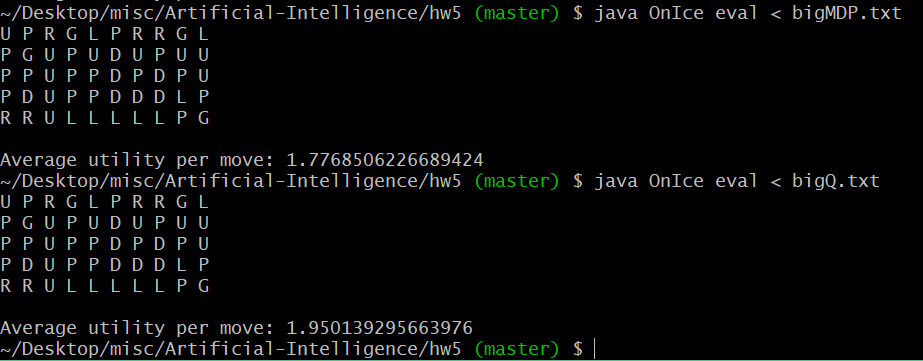
\includegraphics[scale=1.0]{results}

Using the seed provided (5100) for random, I got 1.78 for the average utility per move for the policy created by MDP and 1.95 for the average utility per move for the policy created by Q-Learning. This result was unexpected especially because \textbf{after 10,000 iterations, the policy produced by MDP and Q-Learning were identical}. This difference in utility was probably just a result of the random starting points; with enough iterations, these two average utility per move should converge because they have the exact same policy. In general, the average utility per move should be higher for the MDP than the Q-Learning because MDP uses value iteration and has access to the actual world and rewards. Q-Learning uses less information (does not know the world) but is more efficient than MDP.

\end{document}
